\documentclass[a4paper,11pt]{article}

\usepackage[T1]{fontenc}
\usepackage[utf8]{inputenc}
\usepackage{graphicx}
\usepackage[dvipsnames,table]{xcolor}
\usepackage{hyperref}
\usepackage[a4paper,margin=51pt]{geometry}
\usepackage{tabularx, array}
\usepackage{tikz}
\usepackage{fancyhdr}
\usepackage{multicol}
\usepackage{titlesec}

\titleformat{\section}{\large\scshape\raggedright}{}{0em}{}[\titlerule] % Text formatting of sections
\titlespacing{\section}{0pt}{3pt}{3pt} % Spacing around sections
\graphicspath{{./img/}}
\hypersetup{colorlinks=true, allcolors={black}}

\definecolor{links}{HTML}{000e71}
\definecolor{mail}{HTML}{000e71}
\definecolor{cvcolor}{HTML}{ff9d00}

\def\twodigits#1{\ifnum#1<10 0\fi\the#1}
\def\mydate{\twodigits\day.\twodigits\month.\twodigits\year.}

\setlength{\arrayrulewidth}{1px}
\setlength{\tabcolsep}{7px}
\arrayrulecolor{cvcolor}

%paragraph
\setlength{\parindent}{1em}
\setlength{\parskip}{0.5em}

\title{CV_Goran_Cvijanovic}
\author{Goran Cvijnanović}
\date{\mydate}


\begin{document}
\thispagestyle{fancy}
\fancyhead[L,C,R]{}
\fancyfoot[L]{Created}
\fancyfoot[C]{@}
\fancyfoot[R]{\mydate}
\renewcommand{\headrulewidth}{0pt}
\renewcommand{\footrulewidth}{1pt}

% \tikz[remember picture,overlay] \node[opacity=0.05, xshift=8.45cm, yshift=-3.6cm] at (current page.north west){
\includegraphics[width=97px]{logo}};
{\fontfamily{qag}\selectfont
  \begin{table}[t!]
    \begin{tabularx}{\textwidth}{l|cXr}
      \raisebox{-.5\height}{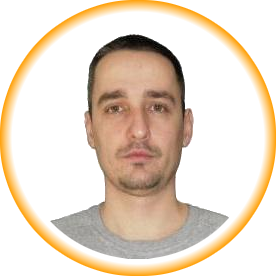
\includegraphics[width=101px]{picture}}&
      \def\arraystretch{1.5}
      \begin{tabular}[c]{c}
        \href{mailto:goran.rs.bg@gmail.com}{\textcolor{mail}{goran.rs.bg@}gmail.com} \\[-2pt]
        \href{tel:0641472353}{\color{links}064\color{black}{/}\color{links}147\color{black}{-}\color{links}23\color{black}{-}\color{links}53} \\[-2pt]
        \href{https://github.com/goranrsbg}{\textcolor{links}{G}it\color{links}{Hub}}
        \href{https://www.linkedin.com/in/goranrsbg}{, \textcolor{links}{Link}ed\textcolor{links}{In}} \\[-2pt]
        November 16, 1982. \\[-2pt]
        Belgrade, Palilula \\[-2pt]
        Category B            
      \end{tabular}
      \def\arraystretch{1}
      &&
      \begin{tabular}[r]{r}
        
\includegraphics[width=157px]{cir_vit}
      \end{tabular}
    \end{tabularx}
  \end{table}
  \begin{center}
    {\fontfamily{phv}\selectfont
      \Large Goran Cvijanović
    }
  \end{center}
  
  \section*{Business Profile}
  
Self-taught programmer, who coded his first lines back in high school and from that point onward fell love with programming, i.e., code writing for solving simple and complex tasks. For years I have been actively actively programming and creating diverse, useful applications.
  
  \section*{Work Experience}
  
  \begin{tabular}{r|l}
    2019 - Current  & Preparation of accounting and other documents, using\\ 
                     & Libre Office Calc/Writer with my custom functions to speed up work\\
                     & and JavaFX applicaton for sending emails (javax.mail).\\
                     & \emph{Freelance}\\
    \multicolumn{2}{c}{} \\
    Past - 2019 & Jobs that had no connection with programming or computers.\\
                     & I dedicated most of my free time to programming.\\
                     & \emph{Smederevo, Beograd}\\
    % ---------------------------------------------------
  \end{tabular}
  
  \section*{Education}
  
  \begin{tabular}{r|l}
    2000 - 2002 & Faculty of Mathematics, \emph{University of Belgrade}\\
    \multicolumn{2}{c}{} \\
    1996 - 2000 & IT Technician, \emph{Tehnical school}, Smederevo\\
    \multicolumn{2}{c}{} \\
    2012 - 2013 & Software developer, \emph{IT Academy}, Belgrade\\ 
    % ---------------------------------------------------
  \end{tabular}
  
  \section*{Technical Skills}
  
  \begin{tabular}{r|l}
    Advanced: & Java, JavaFX, MySql, algorithms, OOP\\
     \multicolumn{2}{c}{} \\
    Intermediate:  & Hibernate, PHP, Laravel, Apache Derby, JS,  HTML, CSS, Sass, Git, Linux/Win\\ 
              & lit-html, Vue.js, Angular, C, Agile, {\LaTeX}, OOBasic/Visula Basic\\

  \end{tabular}
  
  \section*{Selected Portfolio Items}
    
    \begin{tabular}{r|l}
    
      \href{http://www.zvono.nastavnikinformatike.com}{\textcolor{links}{eZvono}} & www.zvono.nastavnikinformatike.com\\
      \href{https://github.com/goranrsbg/HouseOfTheRisingSun}{\textcolor{links}{BB-BB-lokator}} & github.com/goranrsbg/HouseOfTheRisingSun\\
      \href{https://github.com/goranrsbg/files-shuffle}{\textcolor{links}{Shuffle My Files}} & github.com/goranrsbg/files-shuffle\\
      \href{https://github.com/goranrsbg/GRKreator}{\textcolor{links}{Cash account creator}} & github.com/goranrsbg/GRKreator\\
    
    \end{tabular}
    
  \section*{Interests and Activities}

   programming education, technology, open-source, sport (basketball, bowling, pool, swimming),
   mathematics, philosophy, classical music, linux
  
  % \vfill
  % Hvala na izdvojenom vremenu i razumevanju.
}
\end{document}
